% preamble-exam-zh.tex — 共享 preamble
% 用于所有 exam-zh 模板
%
% 样式策略：
%   屏幕 → 语义彩色（蓝=关键想法，红=易错，绿=路线，灰=提示/教师备注）
%   打印 → 自动降级为黑白（通过 print mode 或 monochrome 选项）

\documentclass{exam-zh}

% ---------- 基础配置 ----------
\examsetup{
  page/size = a4paper,
  page/show-head = false,
  page/show-foot = false,
  sealline/show = false,
  font = times,
  math-font = xits,
}

\usepackage{tcolorbox}
\usepackage{needspace}
\usepackage{graphicx}
\usepackage{tikz}
\usetikzlibrary{calc,arrows.meta,intersections}
\tcbuselibrary{skins,breakable}

% ---------- 打印/屏幕颜色切换 ----------
% 用法：\documentclass[monochrome]{exam-zh} 即可切换为纯黑白
% 注意：不要使用 \if@xxx 放在 makeatother 外部；这里改成普通条件名。
\newif\ifeduprintcolor
\eduprintcolortrue

\makeatletter
\@ifclasswith{exam-zh}{monochrome}{\eduprintcolorfalse}{}
\makeatother

% ---------- 语义颜色定义 ----------
% 屏幕：有色彩区分；打印：降级为灰度
\ifeduprintcolor
  % --- 屏幕彩色模式 ---
  \definecolor{edu-blue}{RGB}{47, 82, 122}       % 关键想法
  \definecolor{edu-blue-bg}{RGB}{243, 246, 252}
  \definecolor{edu-red}{RGB}{180, 40, 40}         % 易错提醒
  \definecolor{edu-red-bg}{RGB}{255, 245, 240}
  \definecolor{edu-green}{RGB}{34, 100, 60}       % 路线图
  \definecolor{edu-green-bg}{RGB}{242, 250, 245}
  \definecolor{edu-orange}{RGB}{160, 90, 0}       % 训练目标
  \definecolor{edu-orange-bg}{RGB}{255, 248, 235}
  \definecolor{edu-gray}{RGB}{100, 100, 100}      % 提示/教师备注
  \definecolor{edu-gray-bg}{RGB}{248, 248, 248}
  \definecolor{edu-purple}{RGB}{90, 50, 120}      % 思考题
  \definecolor{edu-purple-bg}{RGB}{248, 244, 252}
\else
  % --- 打印黑白模式 ---
  \definecolor{edu-blue}{gray}{0.15}
  \definecolor{edu-blue-bg}{gray}{0.96}
  \definecolor{edu-red}{gray}{0.25}
  \definecolor{edu-red-bg}{gray}{0.97}
  \definecolor{edu-green}{gray}{0.20}
  \definecolor{edu-green-bg}{gray}{0.97}
  \definecolor{edu-orange}{gray}{0.25}
  \definecolor{edu-orange-bg}{gray}{0.98}
  \definecolor{edu-gray}{gray}{0.40}
  \definecolor{edu-gray-bg}{gray}{0.97}
  \definecolor{edu-purple}{gray}{0.30}
  \definecolor{edu-purple-bg}{gray}{0.98}
\fi
\colorlet{edu-diagram-muted}{edu-gray}

% ---------- 自定义教学环境 ----------
% 共性：enhanced + breakable（跨页不断裂）

% 原题卡片 — 强边框，突出显示
\newtcolorbox{problemcard}{
  enhanced, breakable,
  colback=edu-blue-bg,
  colframe=edu-blue,
  boxrule=1.2pt,
  arc=0pt,
  left=3mm, right=3mm, top=3mm, bottom=3mm,
}

% 解题路线图 — 左边线 + 浅底
\newtcolorbox{routebox}{
  enhanced, breakable,
  colback=edu-green-bg,
  colframe=edu-green!30,
  boxrule=0pt,
  borderline west={2.5pt}{0pt}{edu-green},
  left=3mm, right=3mm, top=3mm, bottom=3mm,
}

% 关键想法 — 蓝色左边线
\newtcolorbox{keyideabox}{
  enhanced, breakable,
  colback=edu-blue-bg,
  colframe=edu-blue!30,
  boxrule=0pt,
  borderline west={2.5pt}{0pt}{edu-blue},
  left=3mm, right=3mm, top=3mm, bottom=3mm,
}

% 易错提醒 — 红色左边线
\newtcolorbox{mistakebox}{
  enhanced, breakable,
  colback=edu-red-bg,
  colframe=edu-red!20,
  boxrule=0pt,
  borderline west={3pt}{0pt}{edu-red},
  left=3mm, right=3mm, top=2.5mm, bottom=2.5mm,
}

% 提示 — 灰色虚线左边线
\newtcolorbox{hintbox}{
  enhanced, breakable,
  colback=edu-gray-bg,
  colframe=edu-gray!20,
  boxrule=0pt,
  borderline west={2pt}{0pt}{edu-gray, dashed},
  left=3mm, right=3mm, top=2mm, bottom=2mm,
}

% 思考题 — 紫色虚线左边线
\newtcolorbox{thinkbox}{
  enhanced, breakable,
  colback=edu-purple-bg,
  colframe=edu-purple!20,
  boxrule=0pt,
  borderline west={2pt}{0pt}{edu-purple, dashed},
  left=2.5mm, right=2.5mm, top=2.5mm, bottom=2.5mm,
}

% 教师备注 — 灰色左边线，小字
\newtcolorbox{teachernote}{
  enhanced, breakable,
  colback=edu-gray-bg,
  colframe=edu-gray!15,
  boxrule=0pt,
  borderline west={2pt}{0pt}{edu-gray!60},
  left=2.5mm, right=2.5mm, top=2.5mm, bottom=2.5mm,
  fontupper=\small,
  colupper=black!60,
}

% 训练目标 — 橙色左边线，小字
\newtcolorbox{traininggoal}{
  enhanced, breakable,
  colback=edu-orange-bg,
  colframe=edu-orange!15,
  boxrule=0pt,
  borderline west={1.5pt}{0pt}{edu-orange},
  left=2mm, right=2mm, top=1mm, bottom=1mm,
  fontupper=\small,
}

% 答题区 — 无边框，纯留白
\newcommand{\answerarea}[1][40mm]{%
  \vspace{2mm}%
  \begin{tcolorbox}[
    enhanced, breakable,
    colback=white,
    colframe=white,
    boxrule=0pt,
    height=#1,
    valign=top,
    bottom=0mm,
    after skip=0mm,
  ]
  \end{tcolorbox}%
}

\newcommand{\diagramcolfigure}[3]{%
  \begin{minipage}[t]{#2}
    \vspace{0pt}\centering
    \includegraphics[width=\linewidth]{\detokenize{#1}}
    \if\relax\detokenize{#3}\relax\else
      \par\vspace{1mm}{\scriptsize\color{edu-diagram-muted}#3}
    \fi
  \end{minipage}%
}

\newcommand{\diagramrowitem}[4]{%
  \begin{minipage}[t]{#2}
    \vspace{0pt}\centering
    \includegraphics[width=\linewidth]{\detokenize{#1}}
    \if\relax\detokenize{#3}\relax\else
      \par\vspace{1mm}{\scriptsize\bfseries #3}
    \fi
    \if\relax\detokenize{#4}\relax\else
      \par\vspace{0.5mm}{\scriptsize\color{edu-diagram-muted}#4}
    \fi
  \end{minipage}%
}

\newcommand{\answerareawithdiagramcol}[4]{%
  \vspace{2mm}%
  \begin{tcolorbox}[
    enhanced, breakable,
    colback=white,
    colframe=white,
    boxrule=0pt,
    height=#1,
    valign=top,
    bottom=0mm,
    after skip=0mm,
  ]
  \begin{minipage}[t]{\dimexpr\linewidth-#3-6mm\relax}
    \vspace{0pt}
  \end{minipage}\hfill
  \diagramcolfigure{#2}{#3}{#4}
  \end{tcolorbox}%
}

\newcommand{\answerareawithdiagram}[4]{%
  \answerareawithdiagramcol{#1}{#2}{#3}{#4}%
}

% ---------- 字体设置 ----------
% exam-zh (ctexbook) already sets CJK fonts via ctex.
% Only override if specific fonts are needed.
% macOS: Songti SC, STHeiti, STFangsong
% Linux: SimSun, SimHei, FangSong

% ---------- 页面设置 ----------
% exam-zh (ctexbook) already loads geometry.
% Override margins if needed:
% \geometry{top=16mm, bottom=16mm, left=14mm, right=14mm}

\examsetup{
  question/show-answer = true,
  fillin/show-answer = true,
  solution/show-solution = show-stay,
}

% ---------- 教师版解答样式 ----------
\newtcolorbox{solutionblock}{
  enhanced, breakable,
  colback=edu-blue-bg,
  colframe=edu-blue!25,
  boxrule=0pt,
  borderline west={2pt}{0pt}{edu-blue!50},
  arc=0pt,
  left=3mm, right=3mm, top=2mm, bottom=2mm,
  before skip=2mm,
  after skip=3mm,
  fontupper=\small,
}

% 解答步骤编号
\newcounter{solstep}
\newcommand{\solstep}[2]{%
  \stepcounter{solstep}%
  \par\medskip
  \noindent\hangindent=6mm
  {\color{edu-blue}\bfseries\textcircled{\scriptsize\thesolstep}\enspace #1}\enspace #2\par
}

\begin{document}

\section*{铅垂线法面积练习}

\section*{一、解答题（每题 8 分，共 48 分）}

\needspace{8\baselineskip}

\begin{problem}[points=8]
  如图，已知 $O(0,0)$，$A(4,2)$，$B(-2,3)$，求 $\triangle OAB$ 的面积。
\begin{center}
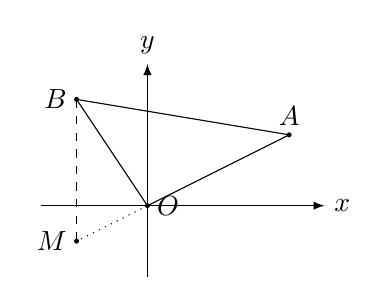
\begin{tikzpicture}[scale=0.45,>=latex]
  \draw[->] (-3,0)--(5,0) node[right]{$x$};
  \draw[->] (0,-2)--(0,4) node[above]{$y$};
  \coordinate (O) at (0,0);
  \coordinate (A) at (4,2);
  \coordinate (B) at (-2,3);
  \coordinate (M) at (-2,-1);
  \draw (O)--(A)--(B)--cycle;
  \draw[dashed] (B)--(M);
  \draw[dotted] (O)--(M);
  \fill (O) circle(2pt) node[right]{$O$};
  \fill (A) circle(2pt) node[above]{$A$};
  \fill (B) circle(2pt) node[left]{$B$};
  \fill (M) circle(2pt) node[left]{$M$};
\end{tikzpicture}
\end{center}

  \answerarea[32mm]
  \setcounter{solstep}{0}
  \begin{solutionblock}
    \textbf{答案：}$8$\par\medskip
    \solstep{求交点}{直线 $OA:y=\frac12x$。过 $B$ 作铅垂线，交 $OA$ 于 $M(-2,-1)$。}
    \solstep{面积}{$BM=4$，横向宽度 $4$，所以 $S=\frac12\times4\times4=8$。}
  \end{solutionblock}
\end{problem}


\needspace{8\baselineskip}

\begin{problem}[points=8]
  如图，已知 $O(0,0)$，$A(2,5)$，$B(-4,1)$，求 $\triangle OAB$ 的面积。
\begin{center}
\begin{tikzpicture}[scale=0.38,>=latex]
  \draw[->] (-5,0)--(3,0) node[right]{$x$};
  \draw[->] (0,-11)--(0,6) node[above]{$y$};
  \coordinate (O) at (0,0);
  \coordinate (A) at (2,5);
  \coordinate (B) at (-4,1);
  \coordinate (M) at (-4,-10);
  \draw (O)--(A)--(B)--cycle;
  \draw[dashed] (B)--(M);
  \draw[dotted] (O)--(M);
  \fill (O) circle(2pt) node[right]{$O$};
  \fill (A) circle(2pt) node[above]{$A$};
  \fill (B) circle(2pt) node[left]{$B$};
  \fill (M) circle(2pt) node[left]{$M$};
\end{tikzpicture}
\end{center}

  \answerarea[32mm]
  \setcounter{solstep}{0}
  \begin{solutionblock}
    \textbf{答案：}$11$\par\medskip
    \solstep{求交点}{直线 $OA:y=\frac52x$。过 $B$ 作铅垂线，交 $OA$ 于 $M(-4,-10)$。}
    \solstep{面积}{$BM=11$，横向宽度 $|2-0|=2$，所以 $S=\frac12\times2\times11=11$。}
  \end{solutionblock}
\end{problem}


\needspace{8\baselineskip}

\begin{problem}[points=8]
  如图，已知 $A(0,1)$，$B(4,5)$，$C(2,0)$，求 $\triangle ABC$ 的面积。
\begin{center}
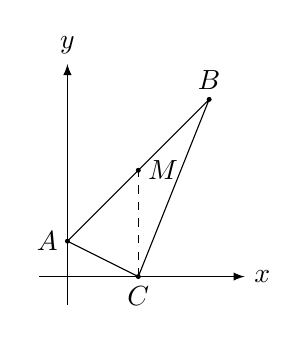
\begin{tikzpicture}[scale=0.45,>=latex]
  \draw[->] (-0.8,0)--(5,0) node[right]{$x$};
  \draw[->] (0,-0.8)--(0,6) node[above]{$y$};
  \coordinate (A) at (0,1);
  \coordinate (B) at (4,5);
  \coordinate (C) at (2,0);
  \coordinate (M) at (2,3);
  \draw (A)--(B)--(C)--cycle;
  \draw[dashed] (C)--(M);
  \fill (A) circle(2pt) node[left]{$A$};
  \fill (B) circle(2pt) node[above]{$B$};
  \fill (C) circle(2pt) node[below]{$C$};
  \fill (M) circle(2pt) node[right]{$M$};
\end{tikzpicture}
\end{center}

  \answerarea[32mm]
  \setcounter{solstep}{0}
  \begin{solutionblock}
    \textbf{答案：}$6$\par\medskip
    \solstep{求交点}{直线 $AB:y=x+1$。过 $C$ 作铅垂线，得 $M(2,3)$。}
    \solstep{面积}{$CM=3$，横向宽度 $4$，所以 $S=\frac12\times4\times3=6$。}
  \end{solutionblock}
\end{problem}


\needspace{8\baselineskip}

\begin{problem}[points=8]
  如图，已知 $A(-2,3)$，$B(4,0)$，$C(6,5)$，求 $\triangle ABC$ 的面积。
\begin{center}
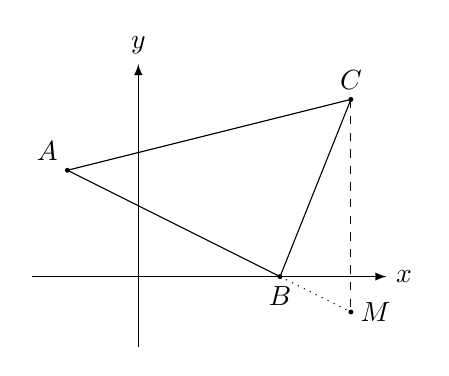
\begin{tikzpicture}[scale=0.45,>=latex]
  \draw[->] (-3,0)--(7,0) node[right]{$x$};
  \draw[->] (0,-2)--(0,6) node[above]{$y$};
  \coordinate (A) at (-2,3);
  \coordinate (B) at (4,0);
  \coordinate (C) at (6,5);
  \coordinate (M) at (6,-1);
  \draw (A)--(B)--(C)--cycle;
  \draw[dashed] (C)--(M);
  \draw[dotted] (B)--(M);
  \fill (A) circle(2pt) node[above left]{$A$};
  \fill (B) circle(2pt) node[below]{$B$};
  \fill (C) circle(2pt) node[above]{$C$};
  \fill (M) circle(2pt) node[right]{$M$};
\end{tikzpicture}
\end{center}

  \answerarea[32mm]
  \setcounter{solstep}{0}
  \begin{solutionblock}
    \textbf{答案：}$18$\par\medskip
    \solstep{求交点}{直线 $AB:y=-\frac12x+2$。过 $C$ 作铅垂线，得 $M(6,-1)$。}
    \solstep{面积}{$CM=6$，横向宽度 $|4-(-2)|=6$，所以 $S=\frac12\times6\times6=18$。}
  \end{solutionblock}
\end{problem}


\needspace{8\baselineskip}

\begin{problem}[points=8]
  如图，已知 $A(0,1)$，$B(4,5)$，点 $P$ 在直线 $y=-x+5$ 上，且 $0\le x_P\le4$。若 $S_{\triangle ABP}=4$，求点 $P$ 的坐标。
\begin{center}
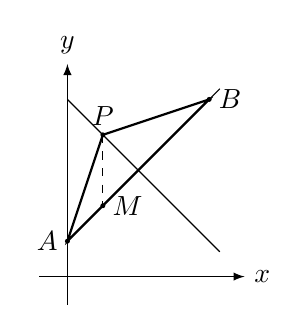
\begin{tikzpicture}[scale=0.45,>=latex]
  \draw[->] (-0.8,0)--(5,0) node[right]{$x$};
  \draw[->] (0,-0.8)--(0,6) node[above]{$y$};
  \draw[domain=0:4.3] plot(\x,{\x+1});
  \draw[domain=0:4.3] plot(\x,{-\x+5});
  \coordinate (A) at (0,1);
  \coordinate (B) at (4,5);
  \coordinate (P) at (1,4);
  \coordinate (M) at (1,2);
  \draw[thick] (A)--(B)--(P)--cycle;
  \draw[dashed] (P)--(M);
  \fill (A) circle(2pt) node[left]{$A$};
  \fill (B) circle(2pt) node[right]{$B$};
  \fill (P) circle(2pt) node[above]{$P$};
  \fill (M) circle(2pt) node[right]{$M$};
\end{tikzpicture}
\end{center}

  \answerarea[40mm]
  \setcounter{solstep}{0}
  \begin{solutionblock}
    \textbf{答案：}$P(1,4)$ 或 $P(3,2)$\par\medskip
    \solstep{设点}{直线 $AB:y=x+1$。设 $P(t,-t+5)$，则 $M(t,t+1)$。}
    \solstep{列方程}{$PM=|4-2t|$，$4=\frac12\cdot4\cdot|4-2t|$，得 $|4-2t|=2$。}
    \solstep{答案}{$t=1$ 或 $t=3$，所以 $P(1,4)$ 或 $P(3,2)$。}
  \end{solutionblock}
\end{problem}


\needspace{8\baselineskip}

\begin{problem}[points=8]
  如图，直线 $AB$ 的解析式为 $y=-x+3$，点 $A,B$ 在这条直线上，且横坐标分别为 $-1,3$。点 $P$ 在直线 $y=2x-2$ 上，且 $x_P>3$。若 $S_{\triangle ABP}=14$，求点 $P$ 的坐标。
\begin{center}
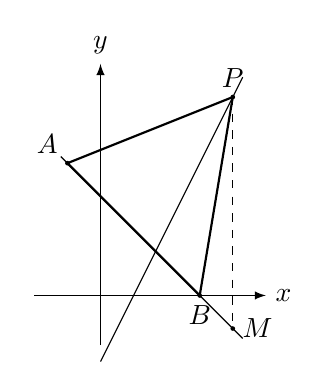
\begin{tikzpicture}[scale=0.42,>=latex]
  \draw[->] (-2,0)--(5,0) node[right]{$x$};
  \draw[->] (0,-1.5)--(0,7) node[above]{$y$};
  \draw[domain=-1.2:4.3] plot(\x,{-\x+3});
  \draw[domain=0:4.3] plot(\x,{2*\x-2});
  \coordinate (A) at (-1,4);
  \coordinate (B) at (3,0);
  \coordinate (P) at (4,6);
  \coordinate (M) at (4,-1);
  \draw[thick] (A)--(B)--(P)--cycle;
  \draw[dashed] (P)--(M);
  \fill (A) circle(2pt) node[above left]{$A$};
  \fill (B) circle(2pt) node[below]{$B$};
  \fill (P) circle(2pt) node[above]{$P$};
  \fill (M) circle(2pt) node[right]{$M$};
\end{tikzpicture}
\end{center}

  \answerarea[40mm]
  \setcounter{solstep}{0}
  \begin{solutionblock}
    \textbf{答案：}$P(4,6)$\par\medskip
    \solstep{设点}{设 $P(t,2t-2)$，同横坐标点 $M(t,-t+3)$。}
    \solstep{列方程}{$PM=|3t-5|$，$14=\frac12\cdot4\cdot|3t-5|$，得 $|3t-5|=7$。}
    \solstep{筛选}{$t=4$ 或 $t=-\frac23$。由 $x_P>3$，取 $t=4$，故 $P(4,6)$。}
  \end{solutionblock}
\end{problem}


\clearpage
\section*{答案速查}




\end{document}
